\documentclass{article}
\usepackage{ucs} 
\usepackage{graphicx}
\usepackage[utf8x]{inputenc} % Включаем поддержку UTF8  
\usepackage[russian]{babel}
\begin{document}
\section{Введение}
\hspace{12pt} Эффект Мёссбауэра, или ядерный гамма-резонанс, заключается в резонансном поглощении ядром гамма-кванта, который был испущен таким же ядром при переходе из возбужденного состояния в основное.
\\
\indent По-видимому, это один из самых <<острых>> физических резонансов из наблюдаемых экспериментально. Действительно, добротность мёссбауэровского резонанса можно оценить через отношение естественной ширины $\Gamma$ 
гамма-перехода ядра к энергии E этого перехода. Для наиболее употребительного в мёссбауэровской спектроскопии гамма-перехода ядра $^{57}Fe$ из возбужденного состояния с энергией E = 14,413 кэВ (период полураспада - 98,1 нс, $\Gamma$ $\approx$ $7\cdot 10^{-9}$ эВ) в основном добротность резонанса достигает величины $1,5\cdot 10^{12}$. В исключительных же случаях добротность мёссбауэрского резонанса оценивается величиной $10^{15}$ для $^{67}Zn$ и даже  $2\cdot 10^{22}$ для $^{107}Ag$. Именно в силу своей высокой добротности мёссбауэровский ядерный гамма-резонанс оказался мощным, а иногда и единственным методом измерения сверхмалых сдвигов энергии ядерных гамма-переходов.
\\
\indent Эффект Мёссбауэра лежит в основе мёссбауэровской спектроскопии, которая является неразрушающим методом исследования химического состава, кристаллической структуры и магнитных свойств конденсированного состояния вещества. Другое название этого метода исследования вещества - ядерная гамма-резонансная спектроскопия, или ЯГР-спектроскопия. Разумеется, с помощью мёссбауэровской спектроскопии можно исследовать только вещества, которые содержат ядра, демонстрирующие эффект Мёссбауэра, а этот эффект наблюдаем далеко не для всех ядер. Кроме того, это физическое явление может быть полезно для прецизионных измерений гамма квантов, например, с его помощью было измерено гравитационное смещение энергии фотонов.
\section{Физический смысл эффекта Мёссбауэра}
\hspace{12pt} Рассмотрим ядро $^{191}Ir$, находящееся в возбужденном состоянии с энергий E = 129 кэВ, из которого оно может перейти в основное состояние в результате испускания $\gamma$-кванта с периодом полураспада $T_{1/2} \approx 10^{-10}$сек. Тогда согласно соотношению неопределенностей энергия возбужденного состояния E известна с погрешностью $${\Delta}E \approx {\hbar}/{\Delta}t = \frac{10^{-27}}{10^{-10}\cdot 1,6 \cdot 10^{-12}} \approx 5 \cdot 10^{-6} \hspace{2pt}eV$$
\hspace{12pt}Чем быстрее происходит высвечивание возбужденного состояния, тем больше неопределенность в значении энергии возбужденного состояния. Только основное состояние стабильного ядра имеет $\Delta$E = 0 и, следовательно, характеризуется строго определенным значением энергии.
\\
\indent Неопределенность в энергии возбужденного состояния приводит к немонохроматичности $\gamma$-излучения, испускаемого при переходе ядра из возбужденного состояния в основное. Эту немонохроматичность принято называть естественной шириной $\Gamma$ линии испускания $\gamma$-излучения. В нашем примере $\Gamma \approx 5\cdot 10^{-6}$ эВ. Это очень малая величина по сравнению с энергией $\gamma$-перехода E = 129 кэВ. Поэтому если бы существовал способ обнаружения изменения энергии на величину порядка естественной ширины линии излучения, то он дал бы возможность измерять энергию с очень высокой относительной точностью, равной $\Gamma/E$. В нашем примере $\Gamma/E = 4\cdot 10^{-11}$. Для более узких линий, т.е для $\gamma$-переходов с большими периодами, значение $\Gamma/E$ должно быть еще меньше.
\\
\indent В принципе обнаружить изменение энергии, равное естественной ширине линии излучения, можно при помощи резонансного поглощения $\gamma$-излучения. Резонансным поглощением $\gamma$-излучения называется процесс возбуждения ядра под действием $\gamma$-квантов, испускаемых этими ядрами при обратных переходах и данного возбужденного состояния в основное.
\\
\indent Процесс резонансного поглощения можно сравнительно легко наблюдать экспериментально, изучая прохождение резонансного $\gamma$-излучения через пластинку из данного вещества. При совпадении энергии $\gamma$-излучения с энергией перехода поглощение резко возрастает, что позволяет заметить очень небольшие изменения энергии вблизи резонансного значения. Однако до 1958 г. этот метод можно было использовать только при достаточно больших ширинах линий.
\\
\indent Дело в том, что при переходе ядра из возбужденного состояния с энергией E в основное состояние испускающийся $\gamma$-квант уносит не всю энергию возбуждения E, а несколько меньшую величину $E_{\gamma_{em}}$, так как часть энергии $T_{nuc}$ идет на отдачу испускающего ядра: 
$$ E_{\gamma_{em}} = E - T_{nuc} < E$$
(сравните с аналогичным явлением в $\alpha$- и $\beta$-распаде).Аналогично для возбуждения ядра до энергии E необходимо $\gamma$-излучение с энергией 
$$ E_{\gamma_{abs}} = E + T_{nuc} > E,$$
где $T_{nuc}$ - энергия отдачи, передаваемая $\gamma$-квантом поглощающему ядру. Таким образом, линия испускания и линия поглощения для одного и того же состояния в данном ядре сдвинуты относительно друг друга на 2$T_{nuc}$

\begin{figure}[h]
\center{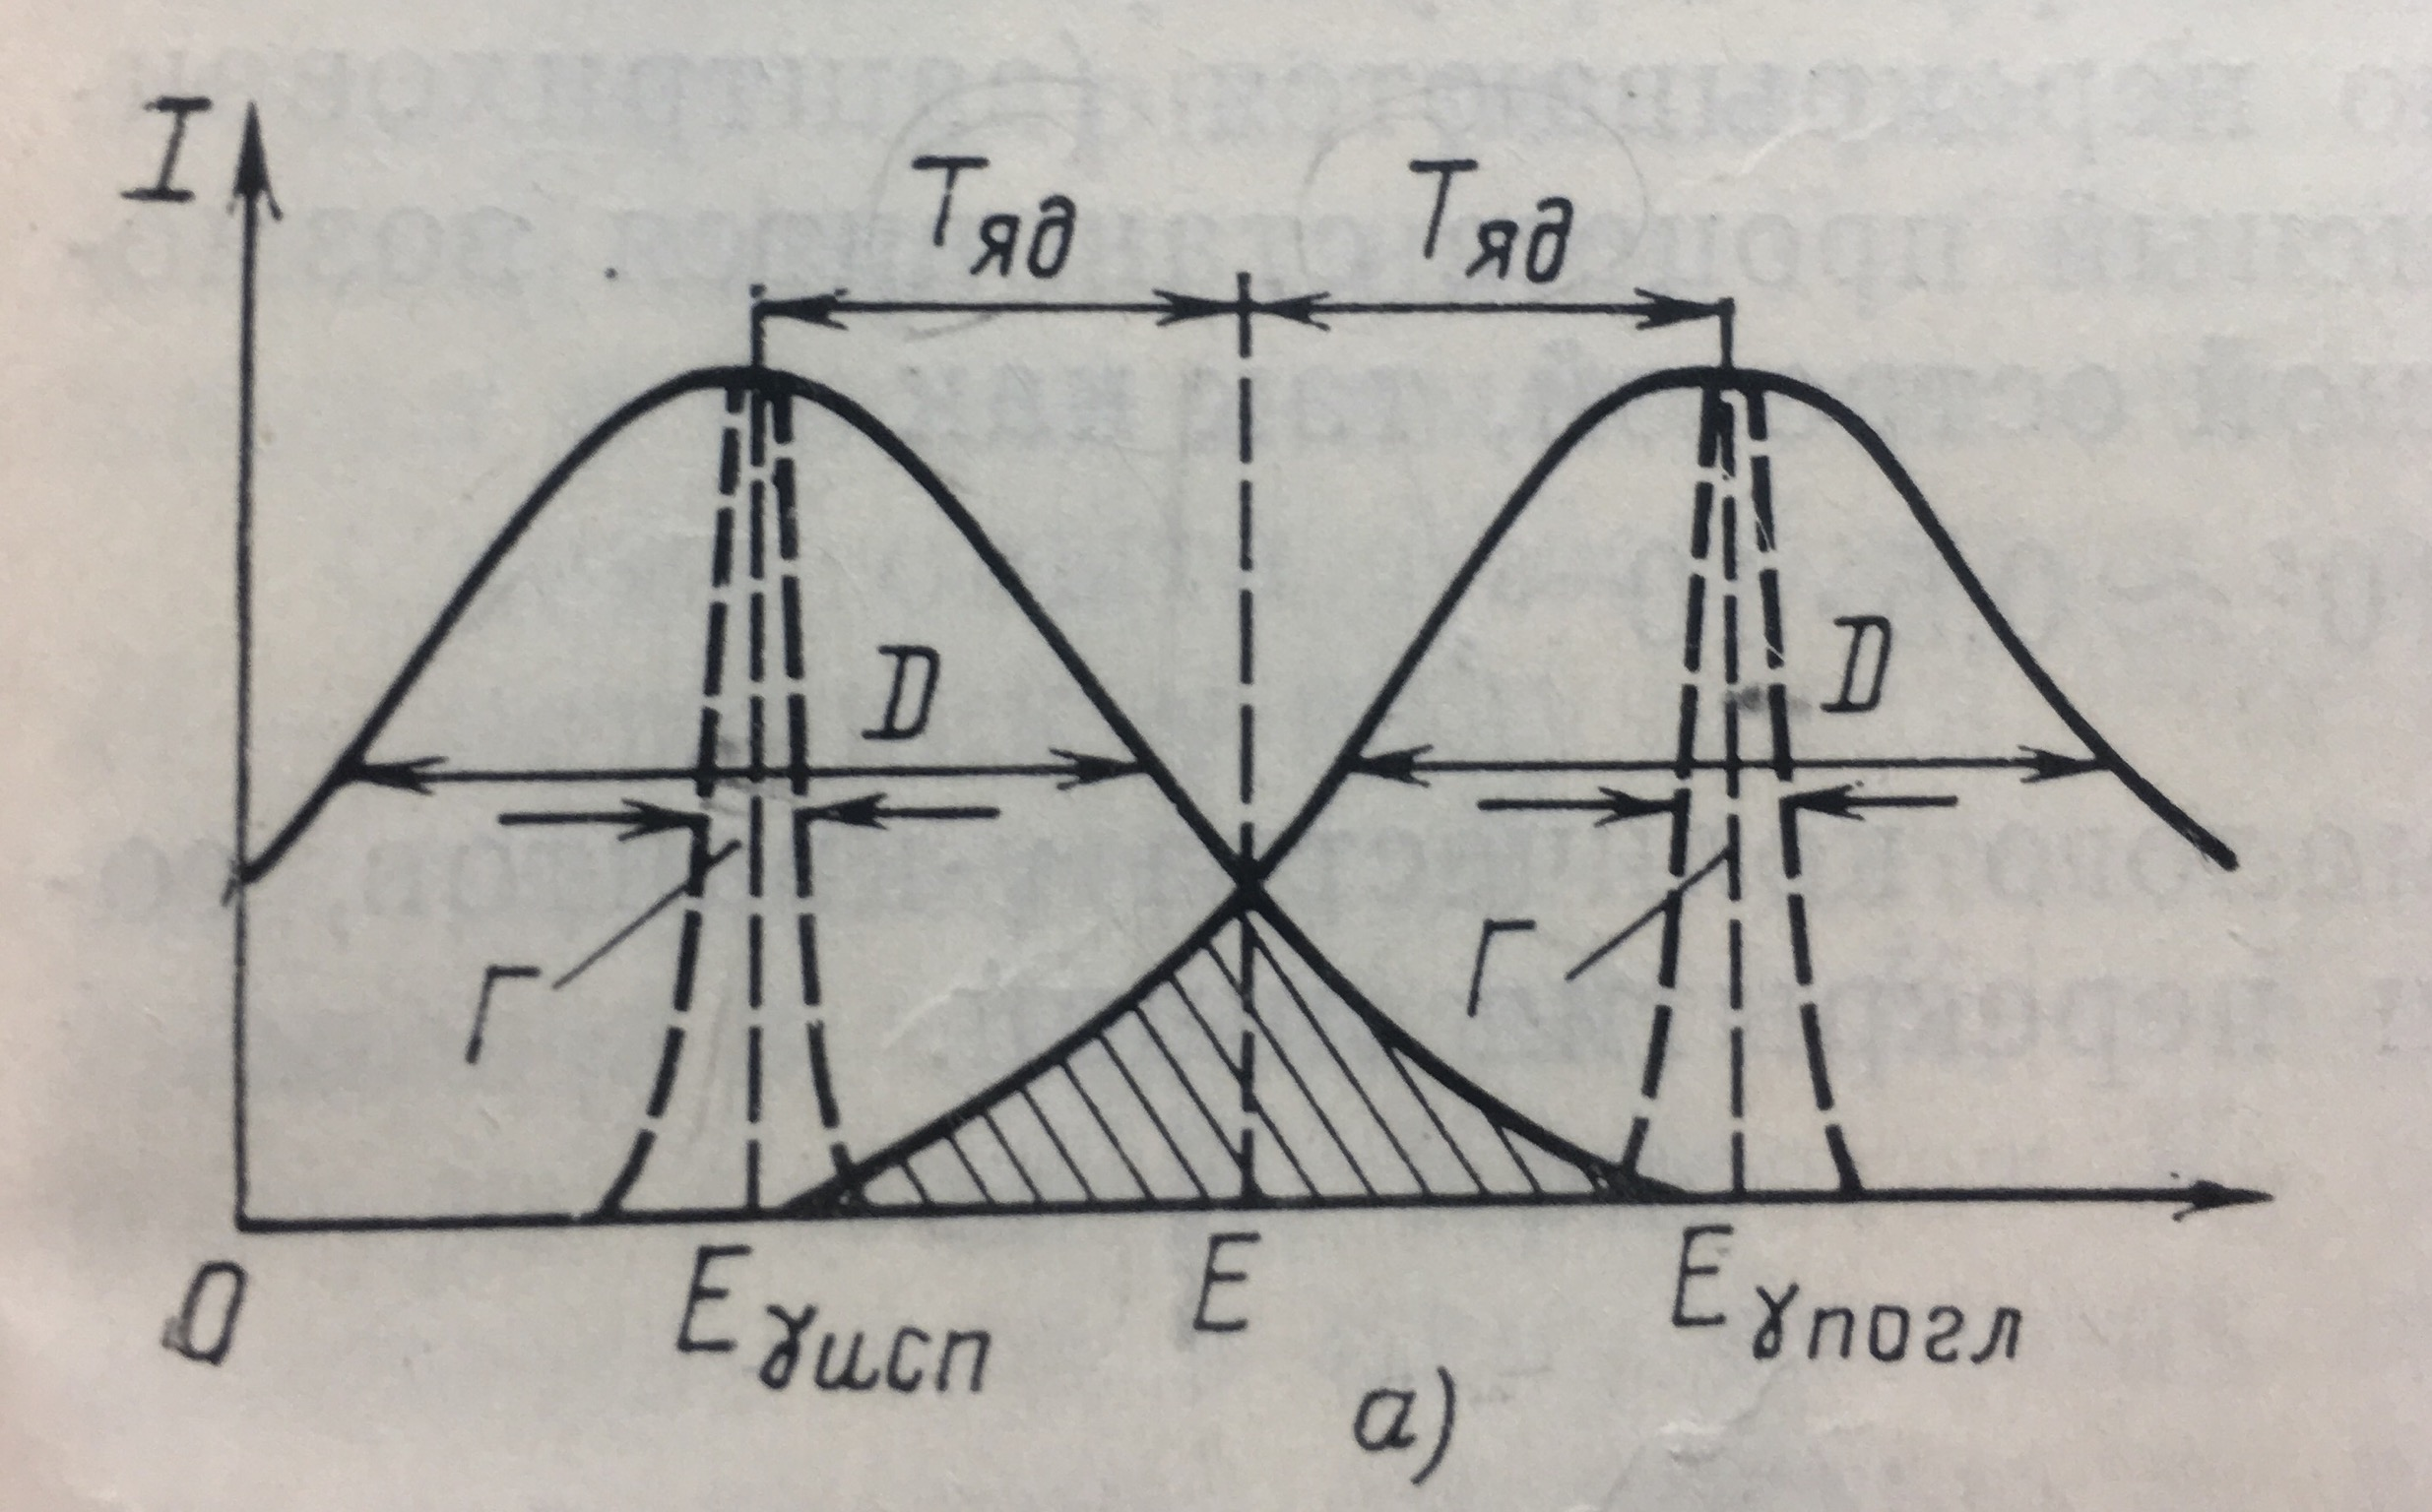
\includegraphics[scale=0.05]{a.jpg}}
\caption{сдвиг}
\label{fig:image}
\end{figure}

\indent Энергию отдачи легко подсчитать, если учесть, что в процессе испускания $\gamma$-кванта должен выполняться закон сохранения импульса $p_{\gamma}$ = $p_{nuc}$:
$$ T_{nuc} = P_{nuc}^{2}/2M_{nuc} = p_{\gamma}^{2}/2M_{nuc} = E_{\gamma}^{2}/2M_{nuc}c^{2} \approx E^{2}/2M_{nuc}c^{2}.$$
\indent Для нашего примера получается очень небольшое значение
$$ T_{nuc} = (1,29\cdot 10^{5})^2/2\cdot 191 \cdot 931 \cdot 10^{6} \approx 0,05 \hspace{2pt}eV$$
однако оно существенно превышает естественную ширину линии излучения $\Gamma$:
$$ T_{nuc} \gg \Gamma $$
\indent Казалось бы отсюда следует абсолютная невозможность резонансного процесса. Однако это неверно потому, что реальная ширина линии испускания(и линии поглощения) определяется не естественной шириной $\Gamma$, а доплеровским уширением:
$$ D = 2\sqrt{T_{nuc}kT^0}$$,
которое при комнатной температуре (T = 300 K, kT = 0,025 эВ) равно
$$ D(300 \hspace{2pt}K) = 2\sqrt{0,05\cdot 0,025} \approx 0,07 \hspace{2pt} eV$$
\indent В связи с тем что $D \approx T_{nuc}$, доплеровски уширенные линии испускания и поглощения частично перекрываются (заштрихованная область на рисунке)  резонансный процесс становится возможен. Правда, он не обладает большой остротой, так как
$$ E/\Gamma = 0,07/1,3 \cdot 10^{5} \approx 0,5 \cdot 10^{-6},$$
и наблюдается только для очень малого количества $\gamma$-квантов, соответствующих небольшой области перекрытия линий.

\section{Два опыта Мёссбауэра}

\end{document}
